\documentclass{article}
\usepackage[utf8]{inputenc}
\usepackage[english]{babel}
\usepackage{amsfonts}
\usepackage{amsthm}
\usepackage{amsmath}
\usepackage{amssymb}
\usepackage{nicefrac}
\usepackage{commath}
\usepackage{dirtytalk}

\usepackage{graphicx}

\newtheorem{theorem}{Theorem}
\newtheorem{es}{Examples}
\newtheorem*{example}{Example}

\newcommand\restr[2]{{% we make the whole thing an ordinary symbol
    \left.\kern-\nulldelimiterspace % automatically resize the bar with \right
    #1 % the function
    \vphantom{\big|} % pretend it's a little taller at normal size
    \right|_{#2} % this is the delimiter
}}

\theoremstyle{definition}
\newtheorem{definition}{Definition}[section]
 
\theoremstyle{remark}
\newtheorem*{remark}{Remark}

\newtheorem{corollary}{Corollary}[theorem]
\newtheorem{lemma}[theorem]{Lemma}

\newtheorem{prop}{Proposition}

\newcommand{\inter}[1]{int(#1)}

\title{MATC34 Exam Study}
\author{Anmol Bhullar}

\begin{document}
    \maketitle

    \textbf{Part 1 Preliminaries to Complex Analysis}

    \textbf{1.1 Basic Properties}
    \begin{definition}
        A \textbf{complex number} takes the form $z = x + iy$ where $x$ and $y$ are real, and $i$ the imaginary 
        number that satisfies $i^2 = -1$. $x$ and $y$ are said to be the \textbf{real part} and the \textbf{imaginary part}
        of $z$, respectively, and we write
        \[ x =\: \text{Re}(z) \qquad\text{and}\qquad\:y=\:\text{Im}(z) \]
        A complex number with zero real part is said to be \textbf{purely imaginary}. The set of all numbers of the form
        $z = x + iy$ is denoted by $\mathbb{C}$.
    \end{definition}

    The natural rules for adding and multiplying complex numbers are:
    \[ z_1 + z_2 = (x_1+x_2) + i(y_1+y_2) \]
    and
    \[ z_1z_2 = (x_1x_2-y_1y_2)+i(x_1y_2+y_1x_2) \]
    $\mathbb{C}$ is a field with these operations so $0$ is the additive identity, $1$ is the multiplicative identity, and $\mathbb{C}$
    has the properties of commutativity, associativity and distributivity.\\
    Addition of  complex numbers can be seen as the addition of two vectors in $\mathbb{R}^2$. Multiplication, however consists of a
    rotation composed with a dilation, where multiplication by $i$ specifically, corresponds to a rotation by an angle of 
    $\nicefrac{\pi}{2}$.

    \begin{definition}
        The notion of length, or absolute value of a complex number is identical to the notion of Euclidean length in $\mathbb{R}^2$.
        Define the \textbf{absolute value} of a complex number $z = x + iy$ by 
        \[ \abs{z} = (x^2 + y^2)^{\frac{1}{2}} \]
        so that $\abs{z}$ is precisely the distance from the origin to the point $(x,y)$. Note this is a norm, so the triangle
        inequality holds as well for all points in $\mathbb{C}$.
    \end{definition}
    \begin{definition}
        The \textbf{complex conjugate} of $z=x+iy$ is defined by
        \[ \overline{z} = x - iy,\]
        and it is obtained by a reflection across the real axis in the plane. One can show that a complex number is real if and only
        if $z = \overline{z}$, and it is purely imaginary if and only if $z = -\overline{z}$.
    \end{definition}
    \begin{lemma}[Results of conjugation]
        One has,
        \[ \text{Re}(z) = \frac{z + \overline{z}}{2}\qquad\text{and}\qquad \text{Im}(z) = \frac{z - \overline{z}}{2i} \]
        Furthermore,
        \[ \abs{z}^2 = z\overline{z}\qquad\text{and as a consequence}\quad \frac{1}{z} = \frac{\overline{z}}{\abs{z}^2} \]
        whenever $z\neq 0$.
    \end{lemma}
    \begin{definition}
        Any non-zero complex number $z$ can be written in \textbf{polar form}
        \[ z = re^{i\theta} \]
        where $r>0$; also $\theta\in\mathbb{R}$ is called the \textbf{argument} of $z$ (defined uniquely up a multiple of $2\pi$)
        and is often denoted by arg$z$, and
        \[ e^{i\theta} = \cos{\theta}+i\sin{\theta}.\]
    \end{definition}
    Since $\abs{e^{i\theta}}=1$ we observe that $r=\abs{z}$, and $\theta$ is simply the angle (with positive counterclockwise
    orientation) between the positive real axis and half-line starting at the origin and passing through $z$.

    \begin{center}
        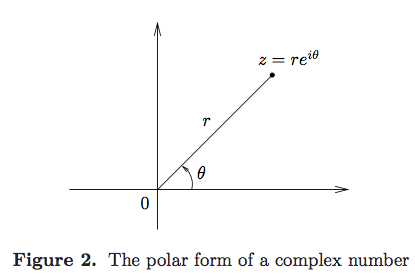
\includegraphics[scale=0.5]{fig2.png}
    \end{center}
    Finally, note that if $z=re^{i\theta}$ and $w=se^{i\varphi}$, then
    \[ zw = rse^{i(\theta+\varphi)}, \]
    so multiplication by a complex number corresponds to a homothety in $\mathbb{R}^2$ (that is, a rotation composed with a dilation).
    
    \newpage

    \textbf{2.1 Functions on the complex plane}
    \begin{definition}
        Let $f$ be a function defined on a set $\Omega$ of complex numbers. We say that $f$ is \textbf{continuous} at the point
        $z_0\in\Omega$ if for every $\epsilon>0$ there exists $\delta>0$ such that whenever $z\in\Omega$ and $\abs{z-z_0}<\Omega$
        then $\abs{f(z)-f(z_0)}<\epsilon$. Equivalently, if for every sequencec $\{z_1,z_2,\hdots\}\subseteq\Omega$ such that
        $\lim z_n = z_0$, then $\lim f(z_n) = f(z_0)$. The function $f$ is said to be continuous on $\Omega$ if it is continuous
        at every point of $\Omega$.
    \end{definition}

    \begin{definition}
        We say that $f$ attains a \textbf{maximum} at the point $z_0\in\Omega$ if
        \[ \abs{f(z)} \leq \abs{f(z_0)}\qquad\text{for all}\:z\in\Omega \]
        with the inequality reversed for the definition of a \textbf{minimum}.
    \end{definition}

    \textbf{2.2 Holomorphic functions}
    \begin{definition}
        Let $\Omega$ be an open set in $\mathbb{C}$ and $f$ a complex-valued function on $\Omega$. The function $f$ is 
        \textbf{holomorphic at the point} $z_0\in\Omega$ if the quotient
        \begin{align}
            \frac{f(z_0+h)-f(z_0)}{h}
        \end{align}
        converges to a limit when $h\to0$. Here $h\in\mathbb{C}$ and $h\neq 0$ with $z_0+h\in\Omega$, so that the quotient is well
        defined. The limit of the quotient, when it exists, is denoted by $f'(z_0)$, and is called the \textbf{derivative 
            of $f$ at $z_0$}:
        \[ f'(z_0) = \lim_{h\to0} \frac{f(z_0+h)-f(z_0)}{h} \]
        The function $f$ is said to be \textbf{holomorphic on} $\Omega$ if $f$ is holomorphic at every point of $\Omega$. If
        $f$ is holomorphic in all of $\mathbb{C}$ we say that $f$ is \textbf{entire}.
    \end{definition}

    \begin{example}
        The function $f(z)=\overline{z}$ is not holomorphic. Indeed, we have
        \[ \frac{f(z_0+h)-f(z_0)}{h} = \frac{\overline{h}}{h} \]
        which has no limit as $h\to 0$, as one can see by first taking $h$ real and then $h$ purely imaginary.
    \end{example}

    \begin{example}
        In terms of real variables, the function $f(z) = \overline{z}$ corresponds to the map $F: (x,y) \mapsto (x,-y)$ which is
        differentiable in the real sense. Its derivative at a point is the linear map given by its Jacobian, the $2\times 2$ matrix
        of partial derivatives of the coordinate functions. In fact, $F$ is linear and is therefore equal to its derivative. 
        This implies $F$ is actually indefinitely differentiable. In particular, the existence of the real derivative need 
        not guarantee that $f$ is holomorphic.
    \end{example}

    \newpage

    \textbf{Cauchy-Riemann Equations}\\

    Associate to each complex-valued function $f = u + iv$ the mapping $F(x,y) = (u(x,y),v(x,y))$ from $\mathbb{R}^2$ to 
    $\mathbb{R}^2$.\\
    Recall that a function $F(x,y) = (u(x,y),v(x,y))$ is said to be differentiable at a point $P_0 = (x_0,y_0)$ if there exists a
    linear transformation $J:\mathbb{R}^2\to\mathbb{R}^2$ such that
    \begin{align}
        \frac{\abs{F(P_0+H)-F(P_0)-J(H)}}{\abs{H}} \to 0\qquad\text{as}\:H\to0, H\in\mathbb{R}^2 
    \end{align}
    Equivalently, we can write
    \[ F(P_0+H) - F(P_0) = J(H) + \abs{H}\Psi(H), \]
    with $\abs{\Psi(H)}\to0$ as $\abs{H}\to0$. The linear transformation $J$ is unique and is called the derivative of $F$ at $P_0$.
    If $F$ is differentiable of $u$ and $v$ exist, and the linear transformation $J$ is described in the standard basis of $\mathbb{R}^2$
    by the Jacobian matrix of $F$
    \[ J = J_F(x,y) = \begin{pmatrix} \nicefrac{\partial{u}}{\partial{x}} & \nicefrac{\partial{u}}{\partial{y}}  \\
            \nicefrac{\partial{v}}{\partial{x}} & \nicefrac{\partial{v}}{\partial{y}} \end{pmatrix} \]
    Consider the limit in (2) when $h$ is first real, say $h=h_1+ih_2$ with $h_2=0$. Then, if we write $z=x+iy$, $z_0=x_0+iy_0$, and
    $f(z) = f(x,y)$, we find that
    \begin{align*}
        f'(z_0) &= \lim_{h_1\to0} \frac{f(x_0+h_1,y_0)-f(x_0,y_0)}{h_1} \\
        &= \frac{\partial{f}}{\partial{x}}(z_0),
    \end{align*}
    where $\nicefrac{\partial}{\partial{x}}$ denotes the usual partial derivative in the $x$ variable. Now taking $h$ purely imaginary,
    say $h = ih_2$, a similar argument yields
    \begin{align*}
        f'(z_0) &= \lim_{h_2\to0} \frac{f(x_0,y_0+h_2)-f(x_0,y_0)}{ih_2} \\
        &= \frac{1}{i} \frac{\partial{f}}{\partial{y}}(z_0),
    \end{align*}
    where $\nicefrac{\partial}{\partial{y}}$ is partial differentiation in the $y$ variable. Therefore, if $f$ is holomorphic we have
    shown that
    \[ \frac{\partial{f}}{\partial{x}} = \frac{1}{i}\frac{\partial{f}}{\partial{y}}. \]
    Writing $f = u+iv$, we find that separating real and imaginary parts and using $\nicefrac{1}{i}=-i$, that the partials of $u$ and
    $v$ exist, and they satisfy the following non-trivial relations
    \[ \frac{\partial{u}}{\partial{x}} = \frac{\partial{v}}{\partial{y}}\qquad\text{and}\qquad
        \frac{\partial{u}}{\partial{y}} = -\frac{\partial{v}}{\partial{x}}. \]
    These are the \textbf{Cauchy-Riemann} equations. We can also say:
    \[ \frac{\partial}{\partial{z}} = \frac{1}{2}\big{(}\frac{\partial}{\partial{x}} + \frac{1}{i}\frac{\partial}{\partial{y}}\big{)}
        \qquad\text{and}\qquad \frac{\partial}{\partial{\overline{z}}} = \frac{1}{2}\big{(}\frac{\partial}{\partial{x}}-
        \frac{1}{i}\frac{\partial}{\partial{y}}\big{)}. \]
    \begin{prop}
        If $f$ is holomorphic at $z_0$, then
        \[ \frac{\partial{f}}{\partial{\overline{z}}}(z_0) = 0\qquad\text{and}\qquad f'(z_0)=\frac{\partial{f}}{\partial{z}}(z_0)=
            2\frac{\partial{u}}{\partial{z}}(z_0). \]
        Also, if we write $F(x,y) = f(z)$, then $F$ is differentiable in the sense of real variables, and
        \[ \text{det}J_F(x_0,y_0) = \abs{f'(z_0)}^2 \]
    \end{prop}
    \begin{theorem}
        Suppose $f = u+iv$ is a complex-valued function defined on an open set $\Omega$. If $u$ and $v$ are continuously differentiable
        and satisfy the Cauchy-Riemann equations on $\Omega$, then $f$ is holomorphic on $\Omega$ and $f'(z) = 
        \nicefrac{\partial{f}}{\partial{z}}$.
    \end{theorem}

    \newpage

    \textbf{2.3 Power Series}
    \begin{example}
        A prime example of a power series is the complex \textbf{exponential} function, which is defined for $z\in\mathbb{C}$ by
        \[ e^z = \sum_{n=0}^{\infty} \frac{z^n}{n!}. \]
    \end{example}
    \begin{definition}
        In general, a \textbf{power series} is an expansion of the form
        \begin{align}
            \sum_{n=0}^{\infty} a_nz^n,
        \end{align}
        where $a_n\in\mathbb{C}$.
    \end{definition}
    \begin{definition}
        Given a power series $\sum_{n=0}^{\infty} a_nz^n$, there exists $0\leq R\leq \infty$ such that:
        \begin{enumerate}
            \item If $\abs{z}<R$ the series absolutely converges.
            \item If $\abs{z}<R$ the series diverges.
        \end{enumerate}
        Moreover, if we use the convention that $\nicefrac{1}{0}=\infty$ and $\nicefrac{1}{\infty} = 0$, then $R$ is given by
        Hadamard's formula
        \[ \nicefrac{1}{R} = \limsup \abs{a_n}^{\nicefrac{1}{n}} \]
        The number $R$ is called the \textbf{radius of convergence} of the power series, and the region $\abs{z}<R$ the 
        \textbf{disc of convergence}.
    \end{definition}

    \begin{example}
        In particular, we have $R=\infty$ in the case of the exponential function. In contrast, the geometric series
        \[ \sum_{n=0}^{\infty} z^n \]
        converges absolutely only in the disc $\abs{z}<1$ (since its sum is equal to the function $\nicefrac{1}{(1-z)}$ which is
        holomorphic in the open set $\mathbb{C}-1$) so $R = 1$ for the geometric series.
    \end{example}

    \begin{remark}
        On the boundary of the disk of the convergence, $\abs{z}=R$, the situation is more delicate as one can have either
        convergence or divergence. For example, the power series $\sum nz^n$ does not converge on any point of the unit circle
        but the power series $\sum \nicefrac{z^n}{n^2}$ converges at every point of the unit circle.
    \end{remark}

    \begin{example}
        The power series of the \textbf{standard trigonometric functions} are defined by
        \[ \cos{z} = \sum_{n=0}^{\infty} (-1)^n\frac{z^n}{(2n)!},\quad\text{and}\quad\sin{z} = 
            \sum_{n=0}^{\infty}(-1)^n\frac{z^{2n+1}}{(2n+1)!}, \]
    \end{example}
    and they agree with the usual cosine and sine of a real argument whenever $z\in\mathbb{R}$. Furthermore, we have the 
    \textbf{Euler formulas} for sine and cosine functions,
    \[ \cos{z} = \frac{e^{iz} + e^{-iz}}{2}\qquad\text{and}\qquad\sin{z} = \frac{e^{iz}-e^{-iz}}{2i} \]

    \begin{theorem}
        The power series $f(z) = \sum_{n=0}^{\infty} a_nz^n$ defines a holomorphic function in its disc of convergence. The derivative
        of $f$ is also a power series obtained by differentiating term by term the series of $f$, that is,
        \[ f'(z) = \sum_{n=0}^{\infty} na_nz^{n-1} \]
        Moreover, $f'$ has the same radius of convergence as $f'$.
    \end{theorem}

    \begin{corollary}
        A power series is infinitely complex differentiable in its disc of convergence, and the higher derivatives are also power series
        obtained by termwise differentation.
    \end{corollary}

    \begin{definition}
        A function $f$ is defined on an open set $\Omega$ is said to be \textbf{analytic} (or have a \textbf{power series expansion})
        at a point $z_0\in\Omega$ if there exists a power series $\sum a_n(z-z_0)^n$ centered at $z_0$, with a positive radius of
        convergence, such that
        \[ f(z) = \sum_{n=0}^{\infty} a_n(z-z_0)^n\qquad\text{for all $z$ in a neighborhood of $z_0$}. \]
        If $f$ has a power series expansion at every point in $\Omega$, we say that $f$ is \textbf{analytic on} $\Omega$.
    \end{definition}

    All holomorphic functions are analytic and vice versa.

    \newpage

    \textbf{3 Integration along curves}

    \begin{definition}
        A \textbf{parameterized curve} is a function $z(t)$ which maps a closed interval $[a,b]\subseteq\mathbb{R}$ to the complex
        plane. We say that the parameterized curve is \textbf{smooth} if $z'(t)$ exists and is continuous on $[a,b]$ and $z'(t)\neq 0$
        for $t\not\in[a,b]$. At the points $t=a$ and $t=b$, the quantities $z'(a)$ and $z'(b)$ are interpreted as one-sided limits
        \[ z'(a) = \lim_{h\to0,h>0} \frac{z(a+h)-z(a)}{h}\qquad\text{and}\qquad z'(b) = \lim_{h\to0,h<0} \frac{z(b+h)-z(b)}{h} \]
        Similarly, we say that the parameterized curve is \textbf{piecewise smooth} if $z$ is continuous on $[a,b]$ and if there
        exist points
        \[ a = a_0 < a_1 < \hdots < a_n = b \]
        where $z(t)$ is smooth in the intervals $[a_k,a_{k+1}]$. Two parameterizations,
        \[ z:[a,b]\to\mathbb{C} \qquad\text{and}\qquad\tilde{z}:[c,d]\to\mathbb{C}, \]
        are \textbf{equivalent} if there exists a continuously differentiable bijection $s\mapsto t(s)$ from $[c,d]$ to $[a,b]$
        so that $t'(s) > 0$ and
        \[ \tilde{z}(s) = z(t(s)). \]
        A smooth or piecewise-smooth curve is \textbf{closed} if $z(a) = z(b)$ for any of its parameterizations. Finally, a smooth
        or piecewise-smooth curve is \textbf{simple} if it is not self-intersecting, that is, $z(t)\neq z(s)$ unless $s=t$. If a
        curve is closed to begin with, then we say that it is simple whenever $z(t)\neq z(s)$ unless $s=t$, or $s=a$ and $t=b$.
    \end{definition}

    \begin{example}
        Consider the circle $C_r(z_0)$ centered at $z_0$ and of radius $r$, which by definition is the set
        \[ C_r(z_0) = \{z\in\mathbb{C}: \abs{z-z_0} = r\}. \]
        The \textbf{positive orientation} (counterclockwise) is the one that is given by the standard parameterization
        \[ z(t) = z_0 + re^{it},\qquad\text{whenever}\:t\in[0,2\pi], \]
        while the \textbf{negative orientation} (clockwise) is given by
        \[ z(t) = z_0 + re^{-it},\qquad\text{whenever}\:t\in[0,2\pi]. \]
        In general, we shall consider a circle with the \textit{positive} orientation.
    \end{example}

    \begin{definition}
        Given a smooth curve $\gamma$ in $\mathbb{C}$ parameterized by $z:[a,b]\to\mathbb{C}$, and $f$ a continuous function on $\gamma$,
        we define the \textbf{integral of $f$ along} $\gamma$ by
        \[ \int_{\gamma} f(z)dz = \int_a^b f(z(t))z'(t)dt. \]
        In order for this to be meaninful, we have to show this integral is \textit{independent} of the parameterization we choose.
        Say that $\tilde{z}$ is an equivalent parameterization as above. Then the change of variables of formula and the chain
        rule imply that
        \[ \int_a^b f(z(t))z'(t)dt = \int_c^d f(z(t(s)))z'(t(s))t'(s)ds = \int_c^d f(\tilde{z}(s))\tilde{z}'(s)ds. \]
        This proves that the integral of $f$ over $\gamma$ is well defined.
    \end{definition}

    \begin{definition}
        By definition, the \textbf{length} of the smooth curve $\gamma$ is
        \[ \text{lenght}(\gamma) = \int_a^b \abs{z'(t)}dt.\]
    \end{definition}

    \begin{prop}
        Integration of continuous functions over curves satisfies the following properties:
        \begin{enumerate}
            \item It is linear, that is, if $\alpha,\beta\in\mathbb{C}$, then
                \[ \int_{\gamma} (\alpha f(z)+\beta g(z))dz = \alpha\int_{\gamma} f(z)dz + \beta\int_{\gamma} g(z)dz.\]
            \item If $\gamma^{-}$ is $\gamma$ with the reverse orientation, then
                \[ \int_{\gamma} f(z)dz = -\int_{\gamma^{-}} f(z)dz. \]
            \item One has the inequality
                \[ \abs{\int_{\gamma} f(z)dz} \leq \sup_{z\in\gamma}\abs{f(z)}\cdot \text{lenght}(\gamma).\]
        \end{enumerate}
    \end{prop}

    \begin{theorem}
        If a continuous function $f$ has a primitive $F$ in $\Omega$, and $\gamma$ is a curve in $\Omega$ that begins at $\omega_1$
        and ends at $\omega_2$, then
        \[ \int_{\gamma} f(z)dz = F(w_2) - F(w_1) \]
    \end{theorem}

    \begin{corollary}
        If $\gamma$ is a closed curve in an open set $\Omega$, and $f$ is continuous and has a primitive in $\Omega$, then
        \[ \int_{\gamma} f(z)dz = 0. \]
    \end{corollary}

    \begin{corollary}
        If $f$ is holomorphic in a region $\Omega$ and $f'=0$, then $f$ is constant.
    \end{corollary}

    \newpage

    \textbf{Part 2 Cauchy's Theorem and Its Applications}

    \textbf{1 Goursat's theorem}

    \begin{theorem}
        If $\Omega$ is an open set in $\mathbb{C}$, and $T\subseteq \Omega$ a triangle whose interior is also contained in $\Omega$,
        then
        \[ \int_T f(z)dz = 0 \]
        whenever $f$ is holomorphic in $\Omega$.
    \end{theorem}

    \begin{corollary}
        If $f$ is holomorphic in an open set $\Omega$ that contains a rectangle $R$ and its interior, then
        \[ \int_R f(z)dz = 0. \]
    \end{corollary}

    \textbf{2 Local existence of primitives and Cauchy's theorem in a disc}
    \begin{theorem}
        A holomorphic function in an open disc has a primitive in that disc.
    \end{theorem}

    \begin{theorem}[Cauchy's theorem for a disc]
        If $f$ is holomorphic in a disc, then
        \[ \int_{\gamma} f(z)dz = 0 \]
        for any closed curve $\gamma$ in that disc.
    \end{theorem}

    \begin{corollary}
        Suppose $f$ is holomorphic in an open set containing the circle $C$ and its interior. Then
        \[ \int_C f(z)dz = 0 \]
    \end{corollary}

    \textbf{3 Evaluation of some integrals}
    
    \begin{example}
        We show that if $\xi\in\mathbb{R}$, then
        \begin{align}
            e^{-\pi\xi^2} = \int_{-\infty}^{\infty} e^{-\pi x^2}e^{-2\pi ix\xi}dx
        \end{align}
        If $\xi = 0$, the formula is precisely the known integral
        \[ 1 = \int_{-\infty}^{\infty} e^{-\pi x^2}dx. \]
        Now suppose that $\xi > 0$, and consider the function $f(z) = e^{-\pi z^2}$, which is entire, and in particular holomorphic
        in the interior of the toy contour
        \begin{center}
            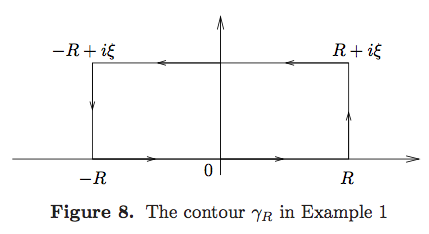
\includegraphics[scale=0.5]{fig8.png}
        \end{center}
        The contour $\gamma_R$ consists of a rectangle with vertices $R,R+i\xi,-R+i\xi,-R$ and the positive counterclockwise
        orientation. By Cauchy's theorem,
        \begin{align}
            \int_{\gamma_R} f(z)dz = 0
        \end{align}
        The integral over the real segment is simply
        \[ \int_{-R}^R e^{-\pi x^2}dx, \]
        which converges to 1 as $R\to\infty$. The integral on the vertical side on the right is
        \[ I(R) = \int_0^{\xi} f(R+iy)idy = \int_0^{\xi} e^{-\pi(R^2+2iRy-y^2)}idy.\]
        This integral goes to 0 as $R\to\infty$ since $\xi$ is fixed and we may estimate it by
        \[ \abs{I(R)} \leq Ce^{-\pi R^2}. \]
        The integral over the vertical segment on the left also goes to 0 as $R\to\infty$ for the same reasons. Finally, the
        integral over the horizontal segment on top is
        \[ \int_{-R}^R e^{-\pi(x+i\xi)^2}dx = -e^{\pi\xi^2}\int_{-R}^R e^{-\pi x^2}e^{-2\pi ix\xi}dx.\]
        Therefore, we find in the limit as $R\to\infty$ that (5) gives
        \[ 0 = 1 - e^{\pi\xi^2}\int_{-\infty}^{\infty} e^{-\pi x^2}e^{-2\pi ix\xi}dx, \]
        and our desired formula is established. In the case $\xi < 0$, we then consider the symmetric rectangle, in the lower
        half plane.
    \end{example}

    \newpage

    \textbf{4 Cauchy's integral formulas}

    \begin{theorem}
        Suppose $f$ is holomorphic in an open set that contains the closure of a disc $D$. If $C$ denotes the boundary circle of this
        disc with the positive orientation, then
        \[ f(z) = \frac{1}{2\pi i}\int_C \frac{f(\zeta)}{\zeta-z}d\zeta \quad\text{for any point}\:z\in D.\]
    \end{theorem}

    \begin{remark}
        Our earlier discussion of toy contours provides simple extensions of the Cauchy integral formula; for instance, if $f$ is
        holomorphic in an open set that contains a (positively oriented) rectangle $R$ and its interior, then
        \[ f(z) = \frac{1}{2\pi i}\int_R \frac{f(\zeta)}{\zeta-z}d\zeta, \]
        whenever $z$ belongs to the interior of $R$. To establisch this result, it suffices to repeat the proof of Theorem 4.1
        replacing the \say{circular} keyhole with a \say{rectangular} keyhole.
    \end{remark}

    \begin{corollary}
        If $f$ is holomorphic in an open set $\Omega$, then $f$ has infinitely many complex derivations in $\Omega$. Moreover,
        if $C\subseteq\Omega$ is a circle whose interior is also contained in $\Omega$, then
        \[ f^{(n)}(z) = \frac{n!}{2\pi i}\int_C \frac{f(\zeta)}{(\zeta-z)^{n+1}}d\zeta \]
        for all $z$ in the interior of $C$.
    \end{corollary}

    \begin{definition}
        The formulas in the above theorem and corollary are said to be the \textbf{Cauchy integral formulas}.
    \end{definition}

    \begin{corollary}[Cauchy's inequalities]
        If $f$ is holomorphic in an open set that contains the closure of a disc $D$ centered at $z_0$ and of radius $R$, then
        \[ \abs{f^{(n)}(z_0)}\leq \frac{n!\norm{f}_C}{R^n}, \]
        where $\norm{f}_C = \sup_{z\in C}\abs{f(z)}$ denotes the supremum of $\abs{f}$ on the boundary circle $C$.
    \end{corollary}

    \begin{theorem}
        Suppose $f$ is holomorphic in an open set $\Omega$. If $D$ is a disc centered at $z_0$ and whose closure is contained in
        $\Omega$. If $D$ is a disc centered at $z_0$ and whose closure is contained in $\Omega$, then $f$ has a power series
        expansion at $z_0$
        \[ f(z) = \sum_{n=0} a_n(z-z_0)^n \]
        for all $z\in D$, and the coefficients are given by
        \[ a_n = \frac{f^{(n)}(z_0)}{n!}\qquad\text{for all}\;n\geq 0 \]
    \end{theorem}

    \begin{corollary}[Liouville's theorem]
        If $f$ is entire and bounded, then $f$ is constant.
    \end{corollary}

    \begin{corollary}
        Every non-constant polynomial $P(z) = a_nz^n + \hdots + a_0$ with complex coefficients has a root in $\mathbb{C}$.
    \end{corollary}

    \begin{corollary}
        Every polynomial $P(z) = a_nz^n + \hdots + a_0$ of degree $n\geq 1$ has precisely $n$ roots in $\mathbb{C}$. If these roots
        are denoted by $\omega_1,\hdots,\omega_n$, then $P$ can be factored as
        \[ P(z) = a_n(z-\omega_1)(z-\omega_2)\cdot\cdot\cdot(z-\omega_n). \]
    \end{corollary}

    \begin{theorem}
        Suppose $f$ is a holomorphic function in a region $\Omega$ that vanishes on a sequence of distinct points with a limit point
        in $\Omega$. Then $f$ is identically 0.
    \end{theorem}

    In other words, if the zeros of a holomorphic function $f$ in the connected set $\Omega$ accumulate \textit{in} $\Omega$, then
    $f = 0$.

    \begin{corollary}
        Suppose $f$ and $g$ are holomorphic in a region $\Omega$ and $f(z) = g(z)$ for all $z$ in some non-empty open subset of 
        $\Omega$ (or more generally for $z$ in some sequence of distinct points with limit point in $\Omega$). Then $f(z)=g(z)$
        throughout $\Omega$.
    \end{corollary}

    Suppose we are given a pair of functions $f$ and $F$ analytic in regions $\Omega$ and $\Omega'$, respectively, with 
    $\Omega\subseteq\Omega'$. If the two functions agree on the smaller set $\Omega$, we say that $F$ is an 
    \textbf{analytic continuation} of $f$ into the region $\Omega'$. The corollary then guarantees that there can only be one such
    analytic continuation, since $F$ is uniquely determined by $f$.

    \newpage

    \textbf{5 Further applications}

    \textbf{5.1 Morera's Theorem}

    \begin{theorem}
        Suppose $f$ is a continuous function in the open disc $D$ such that for any triangle $T$ contained in $D$
        \[ \int_T f(z)dz = 0, \]
        then $f$ is holomorphic.
    \end{theorem}

    \textbf{5.4 Schwarz reflection principle}\\

    Let $\Omega$ be an open subset of $\mathbb{C}$ that is symmetric with respect to the real line, that is
    \[ z\in\Omega\qquad\text{if and only if}\qquad\overline{z}\in\Omega \]
    Let $\Omega^+$ denote the part of $\Omega$ that lies in the upper half plane and $\omega^-$ that part that lies in the lower
    half-plane.\\
    Also, let $I = \Omega\cap\mathbb{R}$ so that $I$ denotes the interior of the part of the boundary of $\Omega^+$ and $\Omega^-$ that
    lies on the real axis. Then we have
    \[ \Omega^+ \cup I \cup \Omega^- = \Omega \]
    and the only interesting case of the next theorem occurs, of cours, when $I$ is non-empty.

    \begin{theorem}[Symmetry principle]
        If $f^+$ and $f^-$ are holomorphic functions in $\Omega^+$ and $\Omega^-$ respectively, that extend continuously to $I$ and
        \[ f^+(x) = f^-(x)\qquad\text{for all}\:x\in I \]
        then the function $f$ defined on $\Omega$ by
        \[ 
            \begin{cases}
                f^+(z) & \text{if}\: z\in\Omega^+,\\
                f^+(z)=f^-(z) & \text{if}\: z\in I,\\
                f^-(z) & \text{if}\: z\in\Omega^-
            \end{cases}
        \]
        is holomorphic on all of $\Omega$.
    \end{theorem}

    \begin{theorem}[Schwarz reflection principle]
        Suppose that $f$ is a holomorphic function in $\Omega^+$ that extends continuously to $I$ and such that $f$ is real-valued
        on $I$. Then there exists a function $F$ holomorphic in all of $\Omega$ such that $F = f$ on $\Omega^+$.
    \end{theorem}

    \newpage

    \textbf{Part 3 Meromorphic Functions and the Logarithm}

    \textbf{1 Zeros and poles}\\
    \begin{definition}
        A \textbf{point singularity} of a function $f$ is a cmoplex number $z_0$ such that $f$ is defined in a neighborhood of $z_0$
        but not at the point $z_0$ itself. We shall also call such points \textbf{isolated singularities}.
    \end{definition}

    \begin{definition}
        A complex number $z_0$ is a \textbf{zero} of the holomorphic function $f$ if $f(z_0) = 0$. In particular, analytic continuation
        shows that zeros of a non-trivial holomorphic function are isolated. In other word, if $f$ is holomorphic in $\Omega$ and
        $f(z_0) = 0$ for some $z_0\in\Omega$, then there exists an open neighborhood $U$ of $z_0$ such that $f(z)\neq 0$ for all
        $z\in U-\{z_0\}$, unless $f$ is identically zero.
    \end{definition}

    \begin{theorem}
        Suppose that $f$ is holomorphic in a connected open set $\Omega$, has a zero at a point $z_0\in\Omega$, and does not vanish
        identically in $\Omega$. Then there exists a neighborhood $U\subseteq \Omega$ of $z_0$, a non-vanishing holomorphic
        function $g$ on $U$, and a unique positive integer $n$ such that
        \[ f(z) = (z-z_0)^ng(z)\qquad\text{for all}\:z\in U. \]
    \end{theorem}

    \begin{definition}
        In the case of the above theorem, we say that $f$ has a \textbf{zero of order} $n$ (or \textbf{multiplicity} $n$) at $z_0$.
        If a zero is of order 1, we say that it is \textbf{simple}. We observe that, quantitatively, the order describes the rate
        at which a function vanishes.
    \end{definition}

    \begin{definition}
        A \textbf{deleted neighborhood} of $z_0$ to be an open disc centered at $z_0$, minus the point $z_0$, that is, the set
        \[ \{z_0: 0 < \abs{z-z_0} < r\} \]
        for some $r>0$. Then, we say that a function $f$ defined in a deleted neighborhood of $z_0$ has a \textbf{pole} at $z_0$,
        if the function $\nicefrac{1}{f}$, defined to be zero at $z_0$ is holomorphic in a full neighborhood of $z_0$.
    \end{definition}

    \begin{theorem}
        If $f$ has a pole at $z_0\in\Omega$, then in a neighborhood of that point there exist a non-vanishing holomorphic function
        $h$ and a unique positive integere $n$ such that
        \[ f(z) = (z-z_0)^{-n}h(z) \]
    \end{theorem}

    \begin{definition}
        The integer $n$ is called the \textbf{order} (or \textbf{multiplicity}) of the pole, and describes the rate at which the
        function grows near $z_0$. If the pole is of order 1, we say that it is \textbf{simple}.
    \end{definition}

    \begin{theorem}
        If $f$ has a pole of order $n$ at $z_0$, then
        \begin{align}
            f(z) = \frac{a_{-n}}{(z-z_0)^n} + \frac{a_{-n+1}}{(z-z_0)^{n-1}} + \hdots + \frac{a_{-1}}{(z-z_0)} + G(z)
        \end{align}
        where $G$ is a holomorphic function in a neighborhood of $z_0$.
    \end{theorem}

    \begin{definition}
        The sum
        \[ \frac{a_{-n}}{(z-z_0)^n} + \frac{a_{-n+1}}{(z-z_0)^{n-1}} + \hdots + \frac{a_{-1}}{(z-z_0)} \]
        is called the \textbf{principal part} of $f$ at the pole $z_0$, and the coefficient $a_{-1}$ is called the \textbf{residue}
        of $f$ at that pole. We write res$_{z_0}f = a_{-1}$.
    \end{definition}

    In the case when $f$ has a simple pole at $z_0$, it is clear that
    \[ \text{res}_{z_0}f = \lim_{z\to z_0} (z-z_0)f(z). \]
    If the pole is of higher order, 
    \begin{theorem}
        If $f$ has a pole of order $n$ at $z_0$, then
        \[ \text{res}_{z_0}f = \lim_{z\to z_0} \frac{1}{(n-1)!}\big{(}\frac{d}{dz}\big{)}^{n-1}(z-z_0)^nf(z). \]
        The theorem is an immediate consequence of formula (6), which implies
        \[ (z-z_0)^nf(z) = a_{-n}+a_{-n+1}(z-z_0) + \hdots + a_{-1}(z-z_0)^{n-1} + G(z)(z-z_0)^n. \]
    \end{theorem}

    \newpage

    \textbf{2 The residue formula}

    \begin{theorem}
        Suppose that $f$ is holomorphic in an open set containing a circle $C$ and its interior, except for a pole at $z_0$ inside
        $C$. Then
        \[ \int_C f(z)dz = 2\pi i \text{res}_{z_0}f. \]
    \end{theorem}

    \begin{corollary}
        Suppose that $f$ is holomorphic in an open set containing a circle $C$ and its interior, except for poles at the points
        $z_1,\hdots,z_N$ inside $C$. Then
        \[ \int_C f(z)dz = 2\pi i\sum_{k=1}^{N} \text{res}_{z_k}f. \]
    \end{corollary}

    \begin{corollary}
        Suppose that $f$ is holomorphic in an open set containing a toy contour $\gamma$ and its interior, except for poles at the
        points $z_1,\hdots,z_N$ inside $\gamma$. Then
        \[ \int_{\gamma} f(z)dz = 2\pi i\sum_{k=1}^{N} \text{res}_{z_k}f. \]
    \end{corollary}

    \begin{definition}
        The identity $\int_{\gamma} f(z)dz = 2\pi i\sum_{k=1}^N \text{res}_{z_k}f$ is referred to as the \textbf{residue formula}.
    \end{definition}

    \textbf{2.1 Examples}

    \newpage

    \textbf{3 Singularities and meromorphic functions}

    \begin{definition}
        Let $f$ be a function holomorphic in an open set $\Omega$ except possibly at one point $z_0$ in $\Omega$. If we can define
        $f$ at $z_0$ in such a way that $f$ becomes holomorphic in all of $\Omega$, we say that $z_0$ is a \textbf{removable}
        singularity for $f$.
    \end{definition}

    \begin{theorem}
        Suppose that $f$ is holomorphic in an open set $\Omega$ except possibly at a point $z_0$ in $\Omega$. If $f$ is bounded on
        $\Omega-\{z_0\}$, then $z_0$ is a removable singularity.
    \end{theorem}

    \begin{corollary}
        Suppose that $f$ has an isolated singularity at the point $z_0$. Then $z_0$ is a pole of $f$ if and only if 
        $\abs{f(z)}\to\infty$ as $z\to z_0$.
    \end{corollary}

    Isolated singularities can belong to one of three categories:
    \begin{itemize}
        \item Removable singularities ($f$ bounded near $z_0$)
        \item Pole singularities ($\abs{f(z)}\to\infty$ as $z\to z_0$)
        \item Essential singularities
    \end{itemize}

    \begin{definition}
        By default, any singularity that is not removable or a pole is defined to be an \textbf{essential singularity}.
    \end{definition}

    \begin{theorem}[Casorati-Weierstrass]
        Suppose $f$ is holomorphic in the punctured disc $D_r(z_0)-\{z_0\}$ and has an essential singularity at $z_0$. Then, the
        image of $D_r(z_0)-\{z_0\}$ under $f$ is dense in the complex plane.
    \end{theorem}

    \begin{definition}
        A function $f$ on an open set $\Omega$ is \textbf{meromorphic} if there exists a sequence of points $\{z_0,z_1,\hdots\}$ that
        has no limit points in $\Omega$, and such that
        \begin{enumerate}
            \item the function $f$ is holomorphic in $\Omega-\{z_0,z_1,\hdots\}$, and
            \item $f$ has poles at the points $\{z_0,z_1,z_2,\hdots\}$.
        \end{enumerate}
    \end{definition}

    \begin{definition}
        If $f$ is holomorphic for all large values of $z$, we consider $F(z) = f(\nicefrac{1}{z})$, which is now holomorphic in
        a deleted neighborhood of the origin. We say that $f$ has a \textbf{pole at infinity} if $F$ has a pole at the origin.
        Similarly, we can speak of $f$ having an \textbf{essential singularity at infinity}, or a \textbf{removable singularity}
        (hence holomorphic) \textbf{at infinity} in terms of the corresponding behaviour of $F$ at 0. A meromorphic function
        in the complex plane that is either holomorphic at infinity or has a pole at infinity is said to be \textbf{meromorphic
            in the extended complex plane}.
    \end{definition}

    \begin{theorem}
        The meromorphic functions in the extended complex plane are the rational functions
    \end{theorem}

    \newpage

    \textbf{4 The argument principle and applications}

    \begin{theorem}[Argument principle]
        Suppose $f$ is meromorphic in an open set containing a circle $C$ and its interior. If $f$ has no poles and never vanishes
        on $C$, then
        \begin{align*}
            \frac{1}{2\pi i}\int_C \frac{f'(z)}{f(z)}dz = (\text{number of zeros of f inside C) minus} \\
            \text{(number of poles of f inside C),}
        \end{align*}
        where the zeros and poles are counted with their multiplicities.
    \end{theorem}

    \begin{corollary}
        The above theorem holds for any toy contours.
    \end{corollary}

    \begin{theorem}[Rouché's theorem]
        Suppose that $f$ and $g$ are holomorphic in an open set containing a circle $C$ and its interior. If
        \[ \abs{f(z)} > \abs{g(z)} \qquad\text{for all}\:z\in\mathbb{C} \]
        then $f$ and $f+g$ have the same number of zeros inside the circle $C$.
    \end{theorem}

    \begin{definition}
        A mapping is said to be \textbf{open} if it maps open sets to open sets.
    \end{definition}

    \begin{theorem}[Open mapping theorem]
        If $f$ is holomorphic and non-constant in a region $\Omega$, then $f$ is open.
    \end{theorem}

    \begin{definition}
        We shall refer to the \textbf{maximum} of a holomorphic function $f$ in an open set $\Omega$ as the maximum of its
        absolute value $\abs{f}$ in $\Omega$.
    \end{definition}

    \begin{theorem}[Maximum modulas principle]
        If $f$ is a non-constant holomorphic function in a region $\Omega$, then $f$ cannot attain a maximum in $\Omega$.
    \end{theorem}

    \newpage

    \textbf{5 Homotopies and simply connected domains}

    \begin{definition}
        Let $\gamma_0$ and $\gamma_1$ be two curves in an open set $\Omega$ with common end-points. So if $\gamma_0(t)$ and
        $\gamma_1(t)$ are two parameterizations defined on $[a,b]$, we have
        \[ \gamma_0(a) = \gamma_1(a) = \alpha \qquad\text{and}\qquad \gamma_0(b) = \gamma_1(b) = \beta \]
        These two curves are said to be \textbf{homotopic in} $\Omega$ if for each $0\leq s\leq 1$ there exists a curve 
        $\gamma_s \subseteq \Omega$, parameterized by $\gamma_s(t)$ defined on $[a,b]$, such that for every $s$
        \[ \gamma_s(a) = \alpha \qquad\text{and}\qquad \gamma_s(b) = \beta, \]
        and for all $t\in[a,b]$
        \[ \gamma_s(t)|_{s=0} = \gamma_0(t) \qquad\text{and}\qquad \gamma_s(t)|_{s=1} = \gamma_1(t) \]
        Moreover, $\gamma_s(t)$ should be jointly continuous in $s\in[0,1]$ and $t\in[a,b]$.
    \end{definition}

    More informally, two curves are homotopic if one curve can be deformed into the other by a continuous transformation without
    ever leaving $\Omega$.

    \begin{theorem}
        If $f$ is holomorphic in $\Omega$, then
        \[ \int_{\gamma_0} f(z)dz = \int_{\gamma_1} f(z)dz \]
        whenever the two curves $\gamma_0$ and $\gamma_1$ are homotopic in $\Omega$.
    \end{theorem}

    \begin{theorem}
        Any holomorphic function in a simply connected domain has a primitive.
    \end{theorem}

    \begin{corollary}
        If $f$ is holomorphic in the simply connected region $\Omega$, then
        \[ \int_{\gamma} f(z)dz = 0 \]
        for any closed curve $\gamma\in\Omega$.
    \end{corollary}

    \newpage

    \textbf{6 The complex logarithm}\\

    If $z=re^{i\theta}$, and we want the logarithm to be the inverse to the exponential, then it is natural to get
    \[ \log{z} = \log{r} + i\theta \]
    Here and below, we use the convention that $\log{r}$ denotes the standard (i.e. real) logarithm of the positive number $r$. The
    trouble with the above definition that $\theta$ is uniquely determined up to an integer multiple of $2\pi$. One choice of this
    range is called a \textbf{branch} or \textbf{sheet} of the logarithm. An example of branch would be the choice 
    $-\pi\leq\:\text{arg}z\leq \pi$.

    \begin{theorem}
        Suppose that $\Omega$ is simply connected with $1\in\Omega$, and $0\not\in\Omega$. Then in $\Omega$ there is a branch
        of the logarithm $F(z) = \log_{\Omega}(z)$ so that
        \begin{enumerate}
            \item $F$ is holomorphic in $\Omega$,
            \item $e^{F(z)} = z$ for all $z\in\Omega$,
            \item $F(r) = \log(r)$ whenever $r$ is a real number and near 1.
        \end{enumerate}
    \end{theorem}

    In other words, each branch $\log_{\Omega}(z)$ is an extension of the standard logarithm defined for positive numbers.

    \begin{definition}
        In the slit plane, $\Omega = \mathbb{C} - \{(-\infty,0]\}$ we have the \textbf{principal branch} of the logarithm
        \[ \log{z} = \log{r} + i\theta \]
        where $z=re^{i\theta}$ with $\abs{\theta}<\pi$. (Here we drop the subscript $\Omega$, and write simply $\log{z}$.)
    \end{definition}

    In general
    \[ \log(z_1z_2) \neq \log(z_1) + \log(z_2). \]

    For the principal branch of the logarithm the following Taylor expansion holds:
    \begin{align}
        \log{(1+z)} = z - \frac{z^2}{2} + \frac{z^3}{3} - \hdots = -\sum_{n=1}^{\infty} (-1)^n\frac{z^n}{n}\quad\text{for}\abs{z}<1.
    \end{align}



\end{document}
